In the problem of \textit{interval selection}, an instance consists of a set of intervals arriving on the real line. Each interval is specified by a starting point $s_i$ and an end point $f_i$, with $s_i < f_i$, and it occupies space $[s_i,f_i)$. The conventional notions of  \textit{intersection}, \textit{disjointness}, and \textit{containment} apply. Two intervals can conflict because of a \textit{partial conflict}, or because of \textit{proper inclusion} (figure \ref{fig:conflicts}). In the latter case, we say that the smaller (larger) interval is subsumed (subsumes) by the other. Each interval $I$ is also associated with a weight $w(I)$. The goal is to output a set of disjoint intervals of maximum weight. We focus on two types of weight functions, \textit{unit} weights where $w(I) = 1$ for all $I$, and \textit{proportional} weights where $w(I) = f_i - s_i$. With unit weights, we want to accept as many intervals as possible, whereas with proportional weights, we want to cover as much of the line as possible.
\begin{figure}[H]
	\centering
	
	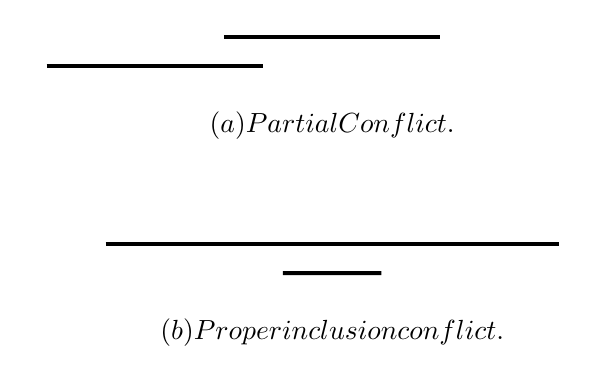
\begin{tikzpicture}[scale=0.75]

	%\node at (-8,-0.5) {$I_{1}$};
	\node[draw=none] (I1a) at (-10,0) {$ $};
	\node[draw=none] (I1b) at (-6,0) {$ $};
	\draw[line width=0.5mm] (I1a) -- (I1b);
	
	
	%\node[draw=none] (d1) at (-3,-1) {$\rvdots$};

	\node[draw=none] (I2a) at (-7,0.5) {$ $};
	\node[draw=none] (I2b) at (-3,0.5) {$ $};
	%\node at (-5,1.5) {$I_{2}$};
	\draw[line width=0.5mm] (I2a) -- (I2b);
	
	\node at (-5,-1) {$(a) \text{ Partial Conflict.}$};
	
	%\node at (-8,-4.5) {$I_{1}$};
	\node[draw=none] (I3a) at (-6,-3.5) {$ $};
	\node[draw=none] (I3b) at (-4,-3.5) {$ $};
	\draw[line width=0.5mm] (I3a) -- (I3b);

 
	
	%\node[draw=none] (d1) at (-3,-1) {$\rvdots$};

	\node[draw=none] (I4a) at (-9,-3) {$ $};
	\node[draw=none] (I4b) at (-1,-3) {$ $};
	%\node at (-5,-3.5) {$I_{2}$};
	\draw[line width=0.5mm] (I4a) -- (I4b);
	
	\node at (-5,-4.5) {$(b) \text{ Proper inclusion conflict}.$};

	\end{tikzpicture} 
	\caption{Types of conflicts.}\label{fig:conflicts}
\end{figure}

The sequence of the intervals arriving online is chosen by an adversary with full knowledge of the algorithm. In the conventional model of \textit{irrevocable decisions}, each accepted interval is final and will be part of the final solution. A well studied relaxation of the model is allowing for \textit{revocable acceptances}, where any new interval may be accepted by displacing any conflicting intervals in the solution, but every rejection is final. This is sometimes also referred to as \textit{preemption}.\\\\
We measure the performance of an online algorithm using \textit{worst case competitive analysis} \cite{BorOnlineBook}. Let $ALG$ denote the total weight of the algorithm's solution, and $OPT$ be the total weight of an optimal solution. An algorithm is strictly $c$-competitive, if for all instances and input permutations, we have that $\frac{OPT}{ALG}\geq c$. We also refer to $ALG$ as the \textit{performance} of the algorithm. Lastly, we will use $ALG$ (respectively $OPT$) to denote the set of intervals in the algorithm's (optimal) solution. The meaning should always be clear from context.\\\\
\textbf{Predictions.} Every interval is associated with a binary prediction that becomes known at the time of the interval's arrival, denoting whether or not that interval is part of some fixed optimal solution. More precisely, $Prd(I)=1$ means interval $I$ is predicted to be optimal, and $Prd(I)=0$ means that it is predicted to not be optimal. Let $\mathcal{I}$ denote the set of all intervals in the instance. We define $\overrightarrow{\textbf{p}} = (Prd(I_1),Prd(I_2),...,Prd(I_{|\mathcal{I}|}))$ to be the binary vector of all the online predictions. Let also $\overrightarrow{\textbf{p}_{+}}$ be the predictions vector when all predictions are accurate, and $\overrightarrow{\textbf{p}_{-}}= \overline{\overrightarrow{\textbf{p}_{+}}}$.\\
\textbf{Error.} Every inaccurate prediction introduces an amount of error. Let $\eta(I)$ be the amount of error introduced by interval $I$. If the prediction of $I$ was accurate, we define $\eta(I)=0$. If $I$ was wrongly predicted to be non-optimal, let $\eta(I) = w(I)$, and if $I$ was wrongly predicted to be optimal, and $\mathcal{C}$ is the set of optimal intervals $I$ conflicts with, let $\eta(I) =\sum_{J\in \mathcal{C}}w(J)\;-\;w(I)$. Let the total error be $\eta = \sum_{I\in\mathcal{I}}\eta(I)$. One may fix any optimal solution to measure the error against. We use $\eta_{max}$ to denote the maximum possible error, i.e. $\eta_{max}=\eta$ when $\overrightarrow{\textbf{p}} = \overrightarrow{\textbf{p}_{-}}$.\\\\
A common approach to evaluate algorithms that use predictions is to focus on an algorithm's \textit{consistency} and \textit{robustness}. We say that an algorithm is $\gamma$-consistent if it is $\gamma$-competitive, whenever the predictions are accurate, i.e. $\overrightarrow{\textbf{p}} = \overrightarrow{\textbf{p}_{+}}$. We say that an algorithm is $\zeta$-robust, if it is $\zeta$-competitive regardless of the accuracy of the predictions. There is usually a trade-off between consistency and robustness, and the goal is to design algorithms with consistency close to $1$, and robustness that is not far worse than the competitiveness of the best predictionless, online algorithm.\\\\
Most of our proofs work by using a \textit{charging argument}, where we map the weight of optimal intervals to the weight of intervals taken by the algorithm, and sometimes error. This charging is usually defined in an online manner, and throughout the execution of the algorithm, we use $\Phi(I)$ to refer to the total amount of charge to interval $I$. In the model of revocable acceptances, we will distinguish between \textit{direct}, and \textit{transfer} charging. Transfer charging ($TC$) occurs at the moment a new interval is accepted by replacing existing intervals, and refers to the amount of charge it inherits because of this. Direct charge ($DC$) takes place afterwards, whenever an interval causes optimal intervals to be rejected. We use $TC(I)$ (respectively $DC(I)$) to denote the amount of transfer (direct) charge of an interval, with $\Phi(I) = TC(I) + DC(I)$.\\
We also use the notion of a \textit{predecessor trace}, which is analogous to Woeginger's \cite{woeginger1994line} \textit{predecessor chain} in th real-time model. If $I$ is an interval in the algorithm's solution, the \textbf{predecessor trace} $\mathcal{P}$ of $I$ is the maximal list of intervals $(P_1,P_2,..,P_k = I)$, such that $P_i$ was at some point accepted by the algorithm, but was later replaced by $P_{i+1}$. 